\usetikzlibrary{calc}
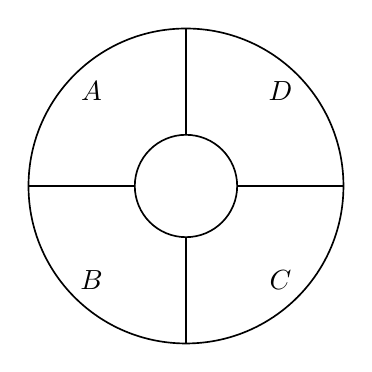
\begin{tikzpicture}[x=1cm,y=1cm,line width=.6pt,font=\normalsize]
\coordinate (O) at (0,0);
\coordinate (T) at (0,2);
\coordinate (Bt) at (0,-2);
\coordinate (L) at (-2,0);
\coordinate (R) at (2,0);
\coordinate (Ti) at (0,0.65);
\coordinate (Bi) at (0,-0.65);
\coordinate (Li) at (-0.65,0);
\coordinate (Ri) at (0.65,0);
\coordinate (labA) at (-1.2,1.2);
\coordinate (labB) at (-1.2,-1.2);
\coordinate (labC) at (1.2,-1.2);
\coordinate (labD) at (1.2,1.2);
\draw (O) circle [radius=2cm];
\draw (O) circle [radius=0.65cm];
\draw (Ti)--(T);
\draw (Bi)--(Bt);
\draw (Li)--(L);
\draw (Ri)--(R);
\node at (labA) {$A$};
\node at (labB) {$B$};
\node at (labC) {$C$};
\node at (labD) {$D$};
\end{tikzpicture}
